\documentclass[11pt]{beamer}
\usepackage[utf8]{inputenc}
\usepackage[T1]{fontenc}
\usepackage{lmodern}
\usepackage[french]{babel}
\usepackage{graphicx}
\usepackage{listings}

\usepackage[export]{adjustbox}

\lstset{
	basicstyle=\ttfamily\scriptsize,
	columns=fullflexible,
	frame=single,
	breaklines=true,
	rulecolor=\color{lightgray},
	literate=
	{á}{{\'a}}1 {é}{{\'e}}1 {í}{{\'i}}1 {ó}{{\'o}}1 {ú}{{\'u}}1
	{Á}{{\'A}}1 {É}{{\'E}}1 {Í}{{\'I}}1 {Ó}{{\'O}}1 {Ú}{{\'U}}1
	{à}{{\`a}}1 {è}{{\`e}}1 {ì}{{\`i}}1 {ò}{{\`o}}1 {ù}{{\`u}}1
	{À}{{\`A}}1 {È}{{\'E}}1 {Ì}{{\`I}}1 {Ò}{{\`O}}1 {Ù}{{\`U}}1
	{ä}{{\"a}}1 {ë}{{\"e}}1 {ï}{{\"i}}1 {ö}{{\"o}}1 {ü}{{\"u}}1
	{Ä}{{\"A}}1 {Ë}{{\"E}}1 {Ï}{{\"I}}1 {Ö}{{\"O}}1 {Ü}{{\"U}}1
	{â}{{\^a}}1 {ê}{{\^e}}1 {î}{{\^i}}1 {ô}{{\^o}}1 {û}{{\^u}}1
	{Â}{{\^A}}1 {Ê}{{\^E}}1 {Î}{{\^I}}1 {Ô}{{\^O}}1 {Û}{{\^U}}1
	{œ}{{\oe}}1 {Œ}{{\OE}}1 {æ}{{\ae}}1 {Æ}{{\AE}}1 {ß}{{\ss}}1
	{ű}{{\H{u}}}1 {Ű}{{\H{U}}}1 {ő}{{\H{o}}}1 {Ő}{{\H{O}}}1
	{ç}{{\c c}}1 {Ç}{{\c C}}1 {ø}{{\o}}1 {å}{{\r a}}1 {Å}{{\r A}}1
	{€}{{\euro}}1 {£}{{\pounds}}1 {«}{{\guillemotleft}}1
	{»}{{\guillemotright}}1 {ñ}{{\~n}}1 {Ñ}{{\~N}}1 {¿}{{?`}}1
}

\usetheme{default}
\begin{document}
	\author{Jean Pommier}
	\title{Introduction à Docker}
	%\subtitle{}
	%\logo{}
	%\institute{}
	%\date{}
	%\subject{}
	%\setbeamercovered{transparent}
	%\setbeamertemplate{navigation symbols}{}
	\begin{frame}[plain]
	\maketitle
	\scriptsize disponible sur \url{https://github.com/jeanpommier/docker-training/}
\end{frame}

\section{Introduction}

\begin{frame}
\frametitle{Un peu d'histoire}
\begin{itemize}
\item Serveurs \textit{old school} : des grosses machines dédiées à une appli
\item Machines virtuelles (VMs) : VMWare, virtualbox, Xen, etc
\item Cloud \& Conteneurs : souple, résilient, jetable
\end{itemize}
\end{frame}

\begin{frame}
\frametitle{Un peu d'histoire}
\framesubtitle{Serveurs \em old school}
\begin{itemize}
	\item une grosse machine, plusieurs applis se partagent le système
	\item un métier : administrateur système
	\vspace{0.5em}
	\item[-] Optimisation des ressources
	\item[-] Évolutivité : \textit{scalability}
	\item[-] Durée de mise en service
\end{itemize}
\end{frame}

\begin{frame}
\frametitle{Un peu d'histoire}
\framesubtitle{Serveurs \em old school}
\begin{itemize}
	\item[] Points de vue
	\begin{itemize}
		\item hébergeurs : un gaspillage de ressources et un frein au développement
		\item sysadmins : un bébé à couver. Pb de suivi de l'état des serveurs. 
		\item développeurs : cycle de vie des applis très long. Pas la main sur le déploiement. Temps de déploiement typique : plusieurs mois.
	\end{itemize}
\end{itemize}
\end{frame}

\begin{frame}
\frametitle{Un peu d'histoire}
\framesubtitle{VMs}
\begin{itemize}
	\item Émulation matérielle
	\item Une machine : plusieurs serveurs virtualisés
	\vspace{0.5em}
	\item[+] Optimisation des ressources
	\item[+] Créer une nouvelle machine est assez rapide
	\item[++] Sécurité : cloisonnement des environnements
	\item[-] Un OS complet dans chaque machine
	\item[-] Volumineux
	\item[-] Attachées à une machine (déplacement lent)
\end{itemize}
\end{frame}

\begin{frame}
\frametitle{Un peu d'histoire}
\framesubtitle{VMs}
\begin{itemize}
	\item[] Points de vue
	\begin{itemize}
		\item hébergeurs : Une nette amélioration. VPS => optimisation des datacenter. + de flexibilité. Débuts du Cloud
		\item sysadmins : Pas une grosse différence. Simplifie la sauvegarde d'un état donné de la machine. Possibilité de prendre des \textit{snapshots}
		\item développeurs : pas de différence majeure. Déploiements potentiellement accélérés.
	\end{itemize}
\end{itemize}
\end{frame}

\begin{frame}
\frametitle{Un peu d'histoire}
\framesubtitle{Conteneurs}
\textbf{Conteneurs} : on allège autant que possible le concept de VM : on utilise le noyau du système hôte et on n'encapsule que le strict nécessaire pour faire tourner l'application.
\vspace{2em}

Un conteneur par service. Une application sera typiquement découpée en plusieurs conteneurs Docker (BD, serveur web, etc)
\end{frame}

\begin{frame}
\frametitle{Un peu d'histoire}
\framesubtitle{Conteneurs}
\begin{itemize}
	\item[++] Optimisation des ressources
	\item[++] Créer une nouvelle machine est très rapide
	\item[+] Sécurité : Isolation relative des environnements
	\item[++] Noyaux commun => petites images 
	\item[++] Microservices
	\item[+++] Iac: Infrastructure as Code. 
	\item[-] Léger surcoût (perfs) de la couche de virtualisation
	\item[-] Stockage : toujours un peu problématique
\end{itemize}
\end{frame}

\begin{frame}
\frametitle{Un peu d'histoire}
\framesubtitle{Conteneurs}
\begin{itemize}
	\item[] Points de vue
	\begin{itemize}
		\item hébergeurs : Full Cloud. Vms jetables. Les serveurs deviennent "anonymes"
		\item sysadmins : change tout. Pas de downtime toléré. Devient "devops". 
		\item développeurs : déploiement simplifié, workflow, devops. Contrepartie : récupère parfois la charge allouée aux sysadmins. Augmentation de la complexité. Temps de déploiement typique : qq dizaines de minutes voire moins.
	\end{itemize}
\end{itemize}
\end{frame}

\begin{frame}
\frametitle{Qu'est-ce que Docker ?}
\begin{itemize}
	\item Un produit de docker.com
	\item Open Source
	\item Une fonctionnalité native Linux, packagée pour la simplicité d'utilisation
	\item Images 
	\begin{itemize}
		\item incrémentielles (Overlay FS) -> réutilisation ! Gain de place
		\item immutables
		\item définies via un fichier Dockerfile => IaC
	\end{itemize}
	\item réseau
	\begin{itemize}
		\item facilité de définir plusieurs réseaux
		\item sécurise facilement les backends
	\end{itemize}
\end{itemize}
\end{frame}

\begin{frame}
\frametitle{Qu'est-ce que Docker ?}
\framesubtitle{Ecosystème : autour de Docker}
\begin{itemize}
	\item Docker hub (\url{https://hub.docker.com/})
	\item Orchestrateurs : (docker-compose), Swarm, Kubernetes, k3c
	\item Outils de gestion de l'infrastructure : Terraform, Rancher, Portainer
	\item Normalisation : OCI (\textit{Open Container Initiative})
	\item Des alternatives : containerd, LXC, rkt, etc
\end{itemize}
\end{frame}

\begin{frame}
\frametitle{Quand utiliser Docker ?}
\framesubtitle{Il fait tout... sauf le café}
\begin{itemize}
	\item Serveurs
	\begin{itemize}
		\item production (\textit{on-premise}, Cloud)
		\item developpement (facilite la reproduction d'un env. de prod en dev)
		\item tester des applis serveur (ex. geOrchestra)
	\end{itemize}
	\item local : lancer un serveur de BD, un serveur web, en une commande
	\item devops
	\begin{itemize}
		\item Compiler une app (\textit{2-stage build})
		\item Automated testing
		\item Deployment
	\end{itemize}
\end{itemize}
\end{frame}

\section{Installation}

\begin{frame}
\frametitle{Installer Docker}
\framesubtitle{Où ça devient sérieux...}
\begin{itemize}
	\item Linux : \textit{RTFM} (\url{https://www.docker.com/get-started})
	\item Windows
	\begin{itemize}
		\item Docker Desktop for Windows : 
		\url{https://docs.docker.com/docker-for-windows/install/}
		\item Redémarrer. Attendre (démarrage Docker très long)
		\item WSL2 (Windows 10 update 2004)
		\item Redémarrer. Attendre.
		\item Redémarrer. Attendre.   ;o)
		\item WSL2  -> \textbf{docker desktop + Linux}
	\end{itemize}
	\item Mac OS : Docker Desktop ?
\end{itemize}
\end{frame}

\section{Pratique}

\begin{frame}[fragile]
\frametitle{Docker pratique : les mains dans le cambouis }
\framesubtitle{Restons simple : un serveur nginx}
\begin{itemize}
	\item Restons traditionnels : 
	\begin{lstlisting}
docker run hello-world	
	\end{lstlisting}
	\item Un serveur web rapide : 
	\begin{lstlisting}
docker run -it --rm -p 82:80 nginx
	\end{lstlisting}
	\item ... avec du contenu : 
	\begin{lstlisting}
docker run -it --rm  -p 82:80 \
-v /home/jean/www:/usr/share/nginx/html nginx
	\end{lstlisting}
\end{itemize}
\end{frame}

\begin{frame}[fragile]
\frametitle{Docker pratique : les mains dans le cambouis }
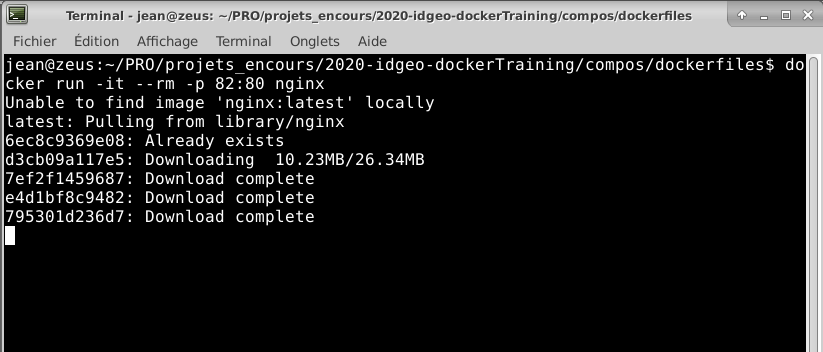
\includegraphics[width=400px]{imgs/docker-run.png}
\end{frame}

\begin{frame}[fragile]
\frametitle{Docker pratique : les mains dans le cambouis }
\framesubtitle{Analysons un peu}
\begin{itemize}
\item Téléchargement des images depuis dockerhub
\item \verb|-p| : correspondance de ports
\item \verb|-v| : monter un volume
\item \verb|--rm| : détruire le conteneur à la sortie
\item \verb|docker run --help|
\end{itemize}
\end{frame}

\begin{frame}[fragile]
\frametitle{Docker pratique : les mains dans le cambouis }
\framesubtitle{Allons un peu plus loin}
\begin{itemize}
	\item relançons notre conteneur : 
	\begin{lstlisting}
docker run -it --rm  -p 82:80 --name nginx \
-v /home/jean/www:/usr/share/nginx/html nginx
	\end{lstlisting}
	\item on va entrer dans le conteneur. Dans une autre console, lancer
	\begin{lstlisting}
docker exec -it  nginx /bin/bash
	\end{lstlisting}
	\item \verb|docker inspect|, un outil bien utile quand la documentation fait défaut
\end{itemize}
\end{frame}

\begin{frame}[fragile]
\frametitle{Docker pratique : les mains dans le cambouis }
\framesubtitle{Bases de données facile}
\begin{itemize}
	\item on peut lancer un serveur de BD sans effort : 
	\begin{lstlisting}
docker run -it --rm  -p 3306:3306 --name mysql mariadb:10.4
	\end{lstlisting}
	\item Quel volume monter pour persister les données ?
	\begin{lstlisting}
docker image inspect --format "{{{{.Config.Volumes}}}}" \
mariadb:10.4
	\end{lstlisting}
	\item Un serveur PostgreSQL ? Facile. Quelle version vous voulez ?
	\begin{lstlisting}
docker run -it --rm  -p 15432:5432 --name pg \ 
-v /tmp/pgdata:/var/lib/postgresql/data postgres:11
	\end{lstlisting}
	\item Vous voulez aussi un PostgreSQL version 9.3 à côté ?
	\begin{lstlisting}
docker run -it --rm  -p 15433:5432 --name pg-9.3 \
-v /tmp/pgdata-9.3:/var/lib/postgresql/data postgres:9.3
	\end{lstlisting}
\end{itemize}
\end{frame}

\begin{frame}[fragile]
\frametitle{Docker pratique : les mains dans le cambouis }
\framesubtitle{Lancer un serveur carto}
\begin{itemize}
\item On peut utiliser une image fournie par la communauté
\begin{lstlisting}
docker run -it --rm  -p 8085:8080 --name geoserver \
-v /tmp/geoserver_datadir:/mnt/geoserver_datadir   \
-v /tmp/geoserver_geodata:/mnt/geoserver_geodata \
pigeosolutions/geoserver:2.15.3
\end{lstlisting}
\item On peut interconnecter la BD PostgreSQL  et GeoServer
\begin{lstlisting}
docker run -it --rm  -p 8085:8080 --name geoserver \
-v /tmp/geoserver_datadir:/mnt/geoserver_datadir \
-v /tmp/geoserver_geodata:/mnt/geoserver_geodata \
--link pg \
pigeosolutions/geoserver:2.15.3
\end{lstlisting}
\end{itemize}
\end{frame}

\begin{frame}[fragile]
\frametitle{Docker pratique : les mains dans le cambouis }
\framesubtitle{Bases de données facile (suite)}
	Vous voulez du PostGIS ?
	\vspace{2em}
	
	Il est temps de fabriquer notre propre image
\end{frame}


\section{Dockerfile}

\begin{frame}[fragile]
\frametitle{Dockerfile}
\framesubtitle{Construire son image}
\begin{itemize}
	\item Fichier texte
	\item définit le contenu de l'image
	\item compilation : \verb|docker build -t jeanpommier/monimage .|
	\item qq commandes principales:
	\begin{description}
		\item[FROM] le point de départ. On construit sur l'existant
		\item[RUN]  exécute une commande (dans la VM). Permet d'installer des librairies, dézipper une archive, bouger/supprimer des fichiers etc
		\item[COPY] copie des fichiers depuis l'ordi
		\item[ADD]  idem, mais permet aussi de copier depuis une URL
		
	\end{description}
	\item[]		Nombreuses autres instructions, cf \url{https://docs.docker.com/engine/reference/builder/}
\end{itemize}
\end{frame}

\begin{frame}[fragile]
\frametitle{Dockerfile}
\framesubtitle{CMD et ENTRYPOINT}
\begin{description}
\item[CMD] la commande lancée par le conteneur au démarrage
\begin{itemize}
	\item format bash
	\item format liste
\end{itemize}
\item[ENTRYPOINT] permet notamment de lancer des scripts d'init
\end{description}

Entrypoints sophistiqués : utilisation de run-parts. Exemple, PostgreSQL
\end{frame}

\begin{frame}[fragile]
\frametitle{Dockerfile}
\framesubtitle{Créer une image PostGIS : v1}
\begin{lstlisting}[title=Dockerfile]
FROM postgres:12

RUN apt-get update && apt-get install postgis -y
# Include datastore setup scripts
COPY ./docker-entrypoint-initdb.d /docker-entrypoint-initdb.d
\end{lstlisting}

\begin{lstlisting}[title=fichier entrypoint]
CREATE EXTENSION POSTGIS;
\end{lstlisting}
\begin{lstlisting}[title=console]
docker build -t jeanpommier/postgis:v1 ./postgis_v1/
docker run -d -it --rm -p 5432:5432 -e POSTGRES_PASSWORD=passwd \
--name pgis jeanpommier/postgis:v1
psql -U postgres -h localhost -p 5432 -d postgres
postgres=# SELECT PostGIS_full_version();
docker stop pgis
\end{lstlisting}
\end{frame}

\begin{frame}[fragile]
\frametitle{Dockerfile}
\framesubtitle{Créer une image PostGIS : v2}
On suit la doc, qui pointe vers un exemple plus complet : 
\url{https://github.com/postgis/docker-postgis/blob/4eb614133d6aa87bfc5c952d24b7eb1f499e5c7c/12-3.0/Dockerfile}
\begin{lstlisting}[basicstyle=\ttfamily\tiny]
FROM postgres:12

LABEL maintainer="PostGIS Project - https://postgis.net"

ENV POSTGIS_MAJOR 2.5
ENV POSTGIS_VERSION 2.5.4+dfsg-1.pgdg100+1

RUN apt-get update \
&& apt-cache showpkg postgresql-$PG_MAJOR-postgis-$POSTGIS_MAJOR \
&& apt-get install -y --no-install-recommends \
postgresql-$PG_MAJOR-postgis-$POSTGIS_MAJOR=$POSTGIS_VERSION \
postgresql-$PG_MAJOR-postgis-$POSTGIS_MAJOR-scripts=$POSTGIS_VERSION \
&& rm -rf /var/lib/apt/lists/*

RUN mkdir -p /docker-entrypoint-initdb.d
COPY ./initdb-postgis.sh /docker-entrypoint-initdb.d/10_postgis.sh
COPY ./update-postgis.sh /usr/local/bin
\end{lstlisting}
\end{frame}

\begin{frame}[fragile]
\frametitle{Docker pratique : les mains dans le cambouis}
\framesubtitle{GeoServer + PostGIS}
On peut interconnecter plusieurs conteneurs

\begin{lstlisting}
docker run -d -it --rm -p 5432:5432 -e POSTGRES_PASSWORD=passwd \
--name pgis jeanpommier/postgis:v1
\end{lstlisting}

On peut interconnecter la BD PostgreSQL  et GeoServer
\begin{lstlisting}
docker run -it --rm  -p 8085:8080 --name geoserver \
-v /tmp/geoserver_datadir:/mnt/geoserver_datadir \
-v /tmp/geoserver_geodata:/mnt/geoserver_geodata \
--link pgis \
pigeosolutions/geoserver:2.15.3
\end{lstlisting}
\end{frame}

\section{docker-compose}

\begin{frame}[fragile]
\frametitle{docker-compose}
\framesubtitle{Les bases de l'orchestration}
\begin{itemize}
	\item publier les ports sur localhost et lier les conteneurs a ses limites
	\item les commandes deviennent très longues
	\item la solution : \textbf{docker-compose}
	\begin{itemize}
		\item assemble la compo dans un fichier texte (yml) 
		\item \textit{As Code} : config persistée dans un fichier
		\item permet de démarrer tous les conteneurs à la fois : \verb|docker-compose up|
		\item versionnable, 
		\item autodocumentéé
		\item IaC
		\item documente facilement un moyen de tester une solution
		\begin{itemize}
			\item wp
			\item georchestra
			\item lizmap
		\end{itemize}
	\end{itemize}
\end{itemize}
\end{frame}

\begin{frame}[fragile]
\frametitle{docker-compose}
\framesubtitle{GeoServer + PostGIS}
\lstinputlisting[numbers=left,basicstyle=\ttfamily\tiny]{../compos/gs.yml}
\end{frame}

\begin{frame}[fragile]
\frametitle{docker-compose}
\framesubtitle{Inclure les infos de compilation}
\begin{lstlisting}[title=gs.yml]
version: '3.1'
services:
  db:
    image: jeanpommier/postgis:v1
    build: ./dockerfiles/postgis_v1
    environment:
...

  geoserver:
    image: pigeosolutions/geoserver:latest
    build: ./dockerfiles/geoserver
...
    
\end{lstlisting}
\begin{lstlisting}[title=console]
docker-compose -f compos/gs.yml build
docker-compose -f compos/gs.yml up -d
\end{lstlisting}

\end{frame}

\begin{frame}[fragile]
\frametitle{docker-compose}
\framesubtitle{Quelques commandes utiles}
\begin{itemize}
	\item verb|docker-compose up|
	\item verb|docker-compose build|
	\item verb|docker-compose ps|
	\item verb|docker-compose logs| : avec l'option -f, suit les logs en temps réel
	\item verb|docker-compose exec|
	\item verb|docker-compose down -v| : supprime les volumes
	\item verb|docker-compose --help|
\end{itemize}
\end{frame}



\end{document}

